\chapter{Results}
\label{chap:results}
\begin{spacing}{1.5}

This chapter presents the results with regards to the evaluation of the retrieval methods applied to the test datasets. We compare various configurations, including query rewriting and reranking, across single-hop and combined datasets.

Briefly restate the test dataset size (400 queries) and the methodology adopted (automatic question generation, retrieval evaluation).
Note the dual evaluation approach (intrinsic retrieval metrics + qualitative)

compare prototype vs. full-scale implementation but HOW????

We conducted a series of experiments to evaluate the performance of different retrieval methods, including dense, BM25, and hybrid approaches. The results are summarized in \autoref{tab:benchmark}, which shows the retrieval effectiveness measured by Recall@5 (R@5), Mean Reciprocal Rank (MRR), Normalised Discounted Cumulative Gain at 5 (nDCG@5), Average Precision at 5 (AP@5), and latency per query.


\section{Prototyping Phase}

A radar plot of the evaluation dimensions in \autoref{fig:proto_results} highlights this profile: strong alignment and topical accuracy, yet with opportunities for improvement in richness and expressivity.

The prototype implementation offered an initial validation of the feasibility of a RAG-based QA system for the Geoportale Nazionale dell’Archeologia. Although limited in scope, it demonstrated that the architecture could effectively combine retrieval and generation within an interactive interface.

The evaluation outcomes (\autoref{fig:proto_results}) indicate a high level of consistency (mean score close to 5) and strong topical relevance ($\approx$ 4.7). Fluency was also rated positively ($\approx$ 4.9), showing that the system could produce linguistically natural answers. By contrast, completeness achieved slightly lower scores ($\approx$ 4.6), suggesting that responses occasionally lacked sufficient depth or coverage of the available information. Overall, the radar profile highlights a system capable of producing reliable and coherent answers, while leaving room for improvement in expressivity and informational richness.

\begin{figure}[H]
  \centering
  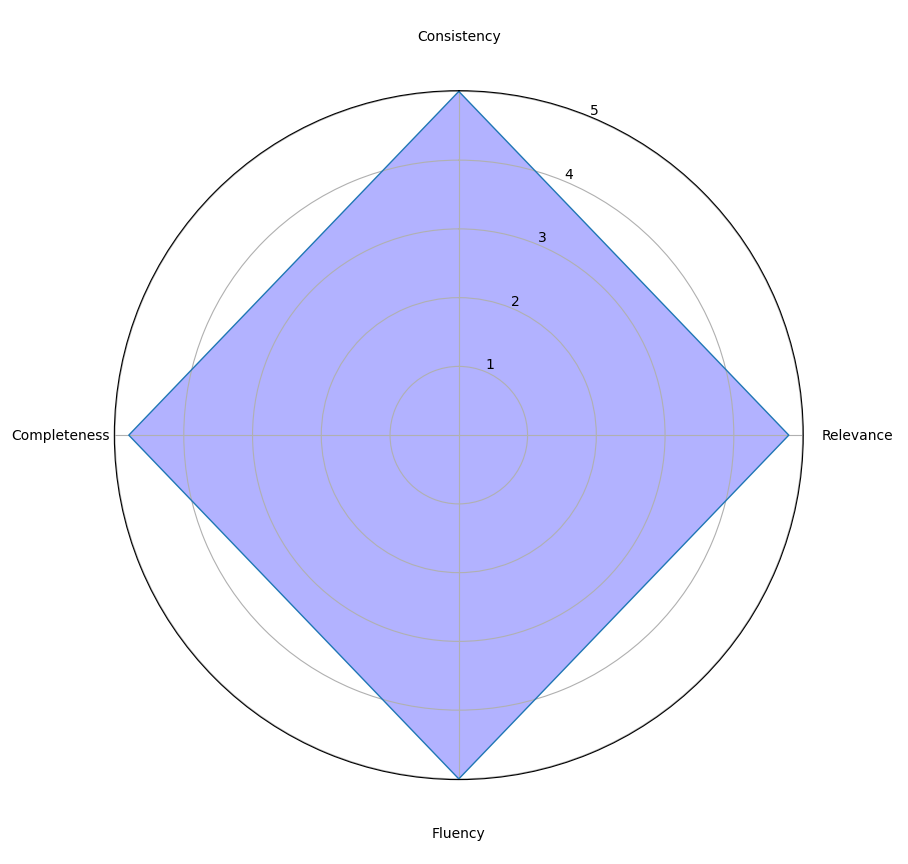
\includegraphics[width=\textwidth]{images/radar.png} 
  \caption{Evaluation results for prototype version of GNA QA system.}
  \label{fig:proto_results}
\end{figure}

Performance testing showed that embedding generation required an average of 31.2 seconds, while query response times averaged 1.26 seconds. Although the latter figure is acceptable for interactive applications, efficiency remains suboptimal compared to production-ready systems, and response delays may accumulate under higher traffic conditions.

\section{Retrieval Performance and Ablation Studies}\label{sec:retrieval_ablation}


\begin{table}[H]
\centering
\resizebox{\linewidth}{!}{%
\setlength{\tabcolsep}{3pt}
\footnotesize
\begin{tabular}{l c c *{10}{c}} % Method, Query rewrite, Rerank, then 10 numeric columns
\toprule
& & & \multicolumn{5}{c}{\textbf{SINGLE-HOP}} & \multicolumn{5}{c}{\textbf{COMBINED (single+multi-hop)}} \\
\cmidrule(lr){4-8}\cmidrule(lr){9-13}
\textbf{Method} & \shortstack[c]{\textbf{Query}\\\textbf{rewrite}} & \textbf{Rerank} & R@5 & MRR & nDCG@5 & AP@5 & Latency & R@5 & MRR & nDCG@5 & AP@5 & Latency \\
\midrule
Dense   &  \xmark     & \xmark & 67.51 & \underline{47.04} & 52.18 & \underline{47.04} & \underline{0.29}  & 50.78 & 48.21 & 53.70 & 34.98 & \underline{0.19} \\
        &  \checkmark & \xmark & 58.07 & 36.76 & 42.09 & 36.76 & 5.98 & 42.64 & 35.41 & 41.32 & 26.24 & 3.10   \\
        & \xmark      &  \checkmark  & 45.47 & 25.41 & 30.36 & 25.41 & 1.30  & 34.57 & 27.71 & 32.90 & 19.48 & 0.82 \\
        & \checkmark  &  \checkmark  & 52.55 & 31.66 & 36.87 & 31.66 & 4.76 & 38.16 & 30.45 & 36.0 & 22.51 & 3.46     \\
\addlinespace
BM25                          & \xmark & \xmark & 65.15 & 43.56 & 48.98 & 43.56 & \textbf{0.001} & 53.09 & \textbf{51.23} & \textbf{57.13} & 35.50 & \textbf{0.001} \\
                              & \checkmark & \xmark & 57.87 & 37.37 & 42.50 & 37.37 & 1.98 & 46.65 & 42.15 & 48.33 & 29.38 & 1.20     \\
                              & \xmark      &  \checkmark  & 45.47 & 25.41 & 30.36 & 25.41 & 1.30  & 34.57 & 27.71 & 32.90 & 19.48 & 0.82 \\
                              & \checkmark  &  \checkmark  & 43.89 & 25.87 & 30.35 & 25.87 & 10.02 & 35.18 & 30.33 & 35.68 & 20.59 & 4.96     \\
Hybrid                        &          &  &  &  &  &  &  &  &  &  &  &      \\
\hspace{0.5em}\textit{+ Weighted RRF}          & \xmark   & \xmark & \underline{69.68} & 46.72 & \underline{52.49} & 46.72 & 0.33  & \textbf{53.98} & \underline{50.93} & \underline{56.92} & \underline{36.15} & 0.32 \\
                              & \checkmark & \xmark & 57.48 & 37.48 & 42.48 & 37.48 & 4.38  & 43.52 & 38.41 & 44.10 & 27.68 & 3.21     \\
                              & \xmark      &  \checkmark  & 43.50 & 24.70 & 29.33 & 24.70 & 1.67  & 33.06 & 26.36 & 31.26 & 18.70 & 0.87 \\
                              & \checkmark  &  \checkmark  & 38.58 & 21.14 & 25.47 & 21.14 & 6.51 & 29.98 & 23.95 & 28.66 & 16.44 & 6.75     \\
\addlinespace
\hspace{0.5em}\textit{+ Score-blend}   & \xmark   & \xmark & \textbf{70.27} & \textbf{48.59} & \textbf{54.02} & \textbf{48.59} & 0.55 & \underline{53.35} & 50.84 & 56.48 & \textbf{36.69} & 0.45     \\
                              & \checkmark & \xmark & 57.67 & 37.17 & 42.31 & 37.17 & 4.57 & 43.61 & 38.16 & 43.87 & 27.52 & 3.99   \\
                              & \xmark      &  \checkmark  & 43.70 & 24.89 & 29.53 & 24.89 & 2.64 & 33.14 & 26.21 & 31.14 & 18.70 & 1.22   \\
                              & \checkmark  &  \checkmark  & 38.58 & 21.47 & 25.72 & 21.47 & 6.44 & 30.13 & 23.98 & 28.82 & 16.55 & 4.8   \\
\bottomrule
\end{tabular}%
}
\caption{Results for different retrieval methods on the test datasets. Best per column is bold and the second-best is underlined. Latency is measured in seconds per query. Reranking is performed using the \textit{cross-encoder/ms-marco-MiniLM-L-6-v2} model.}
\label{tab:benchmark}
\end{table}

Provide a short interpretation — e.g., which configuration excels in which scenario, trade-offs between speed and accuracy, and performance differences between single-hop and combined datasets.

\section{Qualitative Analysis}
Results showed that:

65\% of answers were rated as “Relevant”,

25\% as “Partially relevant”,

10\% as “Not relevant”.

Feedback indicated that relevance dropped when:

the query used ambiguous phrasing,

or too few document chunks were retrieved due to vector sparsity.

Users appreciated:

the traceability of answers via citations,

the lightweight UI,

and the multilingual support.


Include observations about citation traceability, coherence of generated answers.

\section{Summary of Findings}
Neutral recap of what the system achieved (e.g., scalability, stability, acceptable latency).

Highlight consistency (or not) in performance with growing dataset size.

\end{spacing}